% !TeX root = thoughts.tex
\section{Simple linear systems}
In a first analysis a simple linear system is considered, which allows us to get a grip on what is happening behind the scenes. A first analysis will be done on a two dimensional system given by the following linear system;
\begin{gather}
	\begin{pmatrix}
	d_1\\
	d_2
	\end{pmatrix}
	=
	\begin{pmatrix}
	1 & 0\\
	0 & 2\\
	\end{pmatrix}
	\begin{pmatrix}
	q_1\\q_2
	\end{pmatrix}.
\end{gather}
For our synthetic data I choose $q_1 = 1$ and $q_2 = 3$. Prior information and measurement uncertainty all have an impact on posterior exploration, but for now I will set some arbitrary values. Our prior I synthetically set to have all means of 2 and standard deviations of 1. Measurement errors are chosen to be uncorrelated and having a standard deviation of 0.5.


\begin{figure}
	\centering
	\begin{subfigure}{.5\textwidth}
		\centering
		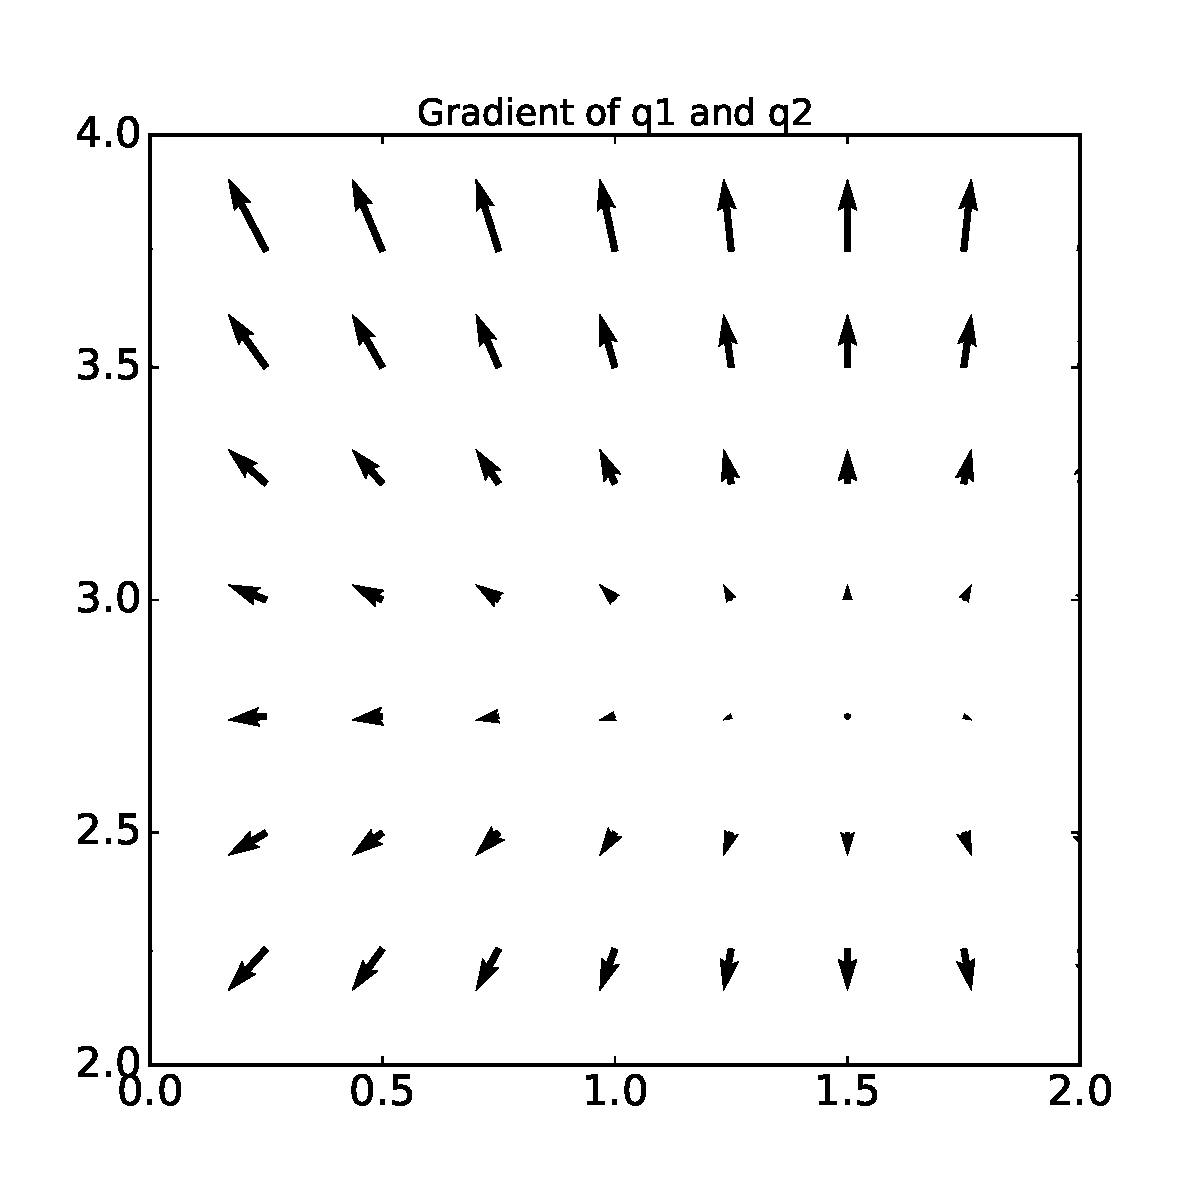
\includegraphics[width=\textwidth]{simple-linear-system/figures/gradient_2d_narrow_prior}
		\caption{Gradient with standard deviation $\sigma = 1$}
		\label{fig:linear_system.prior_influence.narrow}
	\end{subfigure}%
	\begin{subfigure}{.5\textwidth}
		\centering
		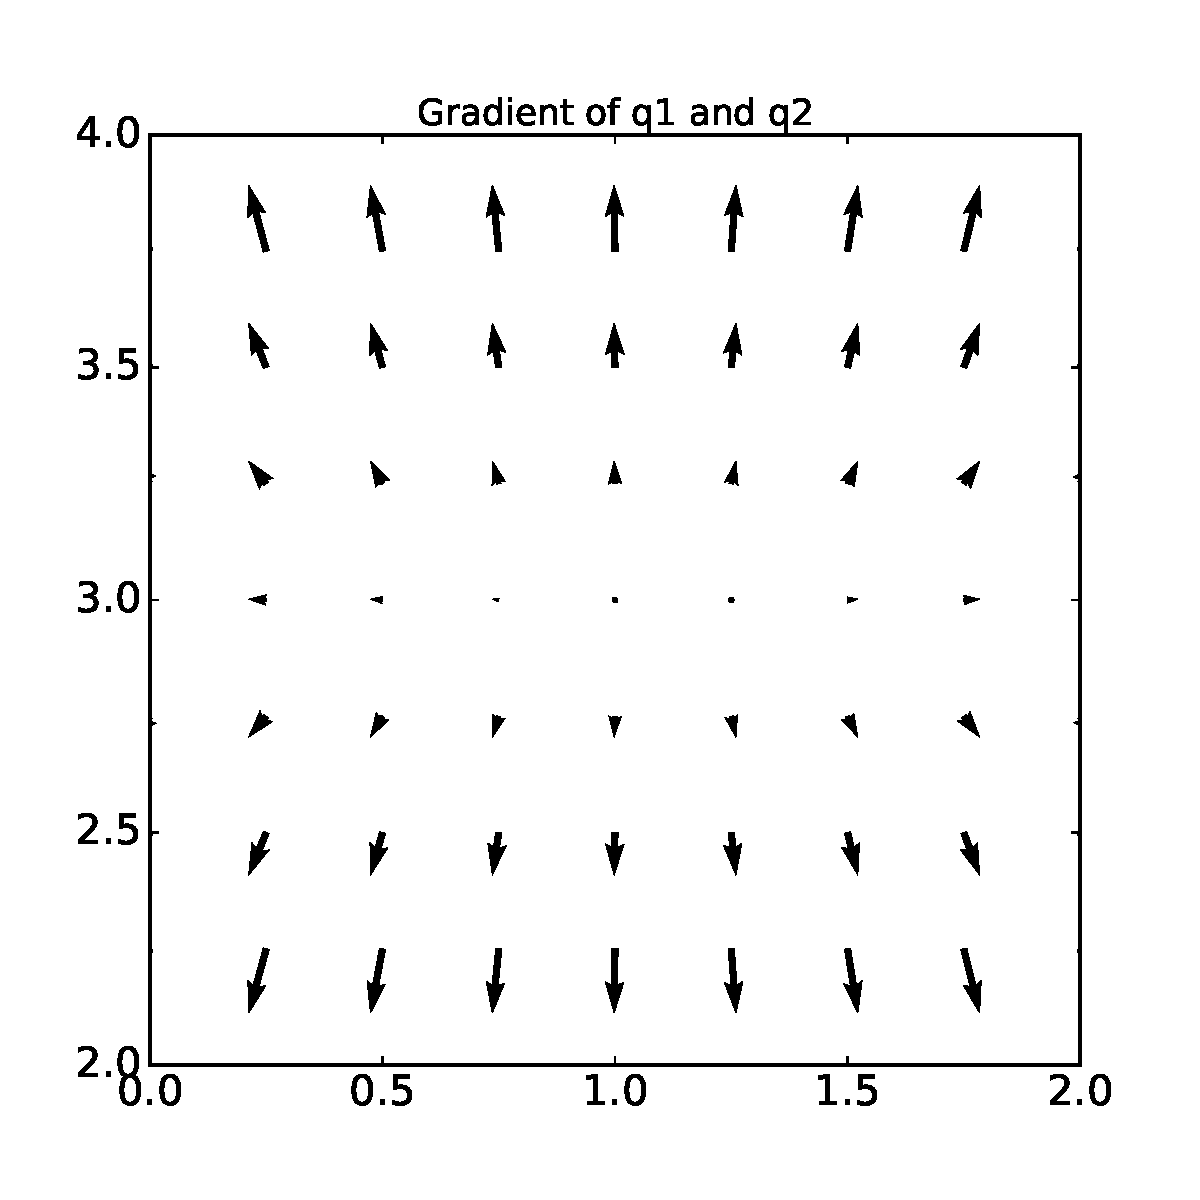
\includegraphics[width=\textwidth]{simple-linear-system/figures/gradient_2d_wide_prior}
		\caption{Gradient with standard deviation $\sigma = 5$}
		\label{fig:linear_system.prior_influence.wide}
	\end{subfigure}
	\caption{Normalized gradient of 2D misfit functionals with differently confined prior information. The means of the prior are for both parameters 2. It is obvious that decreasing the standard deviation for all parameters means that we increase the importance of the prior over the data, `pulling' the minimal gradient more towards the prior mean. Similar effects can be attained with increasing the magnitude of the data covariance matrix. Together, these matrices finely tune the minimum of the misfit function. Choosing well informed data and parameter covariace matrices is essential to meaningful \gls{HMC} sampling.}
	\label{fig:linear_system.prior_influence}
\end{figure}
